\section{Implementing Probes for Data Collection and Analysis}\label{sec:probes_implementation}

In the previous section, we discussed how the single source of truth works and how probes are registered and integrated with it. In this section, we will focus on the implementation of probes to demonstrate the functionality of the framework and validate the scenarios outlined in~\ref{ch3:validation_roadmap}.  

We will cover only the key aspects of the implementation to provide a clear understanding of the process. For those interested in exploring the complete implementation in detail, the full source code is available at~\citep{gh_reverse_engr_awan}.

For each node and edge, we have implemented classes to keep the code consistent and ensure that all objects follow the same structure. We have also created classes to define relationships between nodes, ensuring that the data remains consistent for similar objects.

\subsection{Implementation of probes related to authors and version control}

In section~\ref{ch3-sec:technical_validation_strategy}, we discussed that an effective way to retrieve data related to authors and their contributions is by utilizing a version control system. Version control systems inherently track all changes made to a codebase and store this information within the ``.git'' directory, which is typically hidden. This directory contains the complete history of modifications, including details about contributors, timestamps, and commit messages, making it a reliable source for extracting author-related data.

We have several Python scripts to extract information from a Git repository. These scripts analyze data such as the relationship between two authors based on the number of files they have collaborated on, identifying all authors who worked on a method and determining the top contributor among them, and listing the authors of each file.

Each script relies on the .git file and uses the Javalang library \citep{javalang} to parse Java source code. Javalang helps navigate Java code structure using an Abstract Syntax Tree (AST), making it easier to extract relevant information.

After parsing the Java source code, we extract details about authors, their contributions, and line numbers using the git blame command. Git is a free and open-source distributed version control system \citep{git}. More details about git blame and its usage can be found in the official documentation \citep{git-blame}.

Once the author information is extracted, it is stored in a JSON file and sent to SST for further processing and analysis.

\begin{figure}[H]
    \centering
    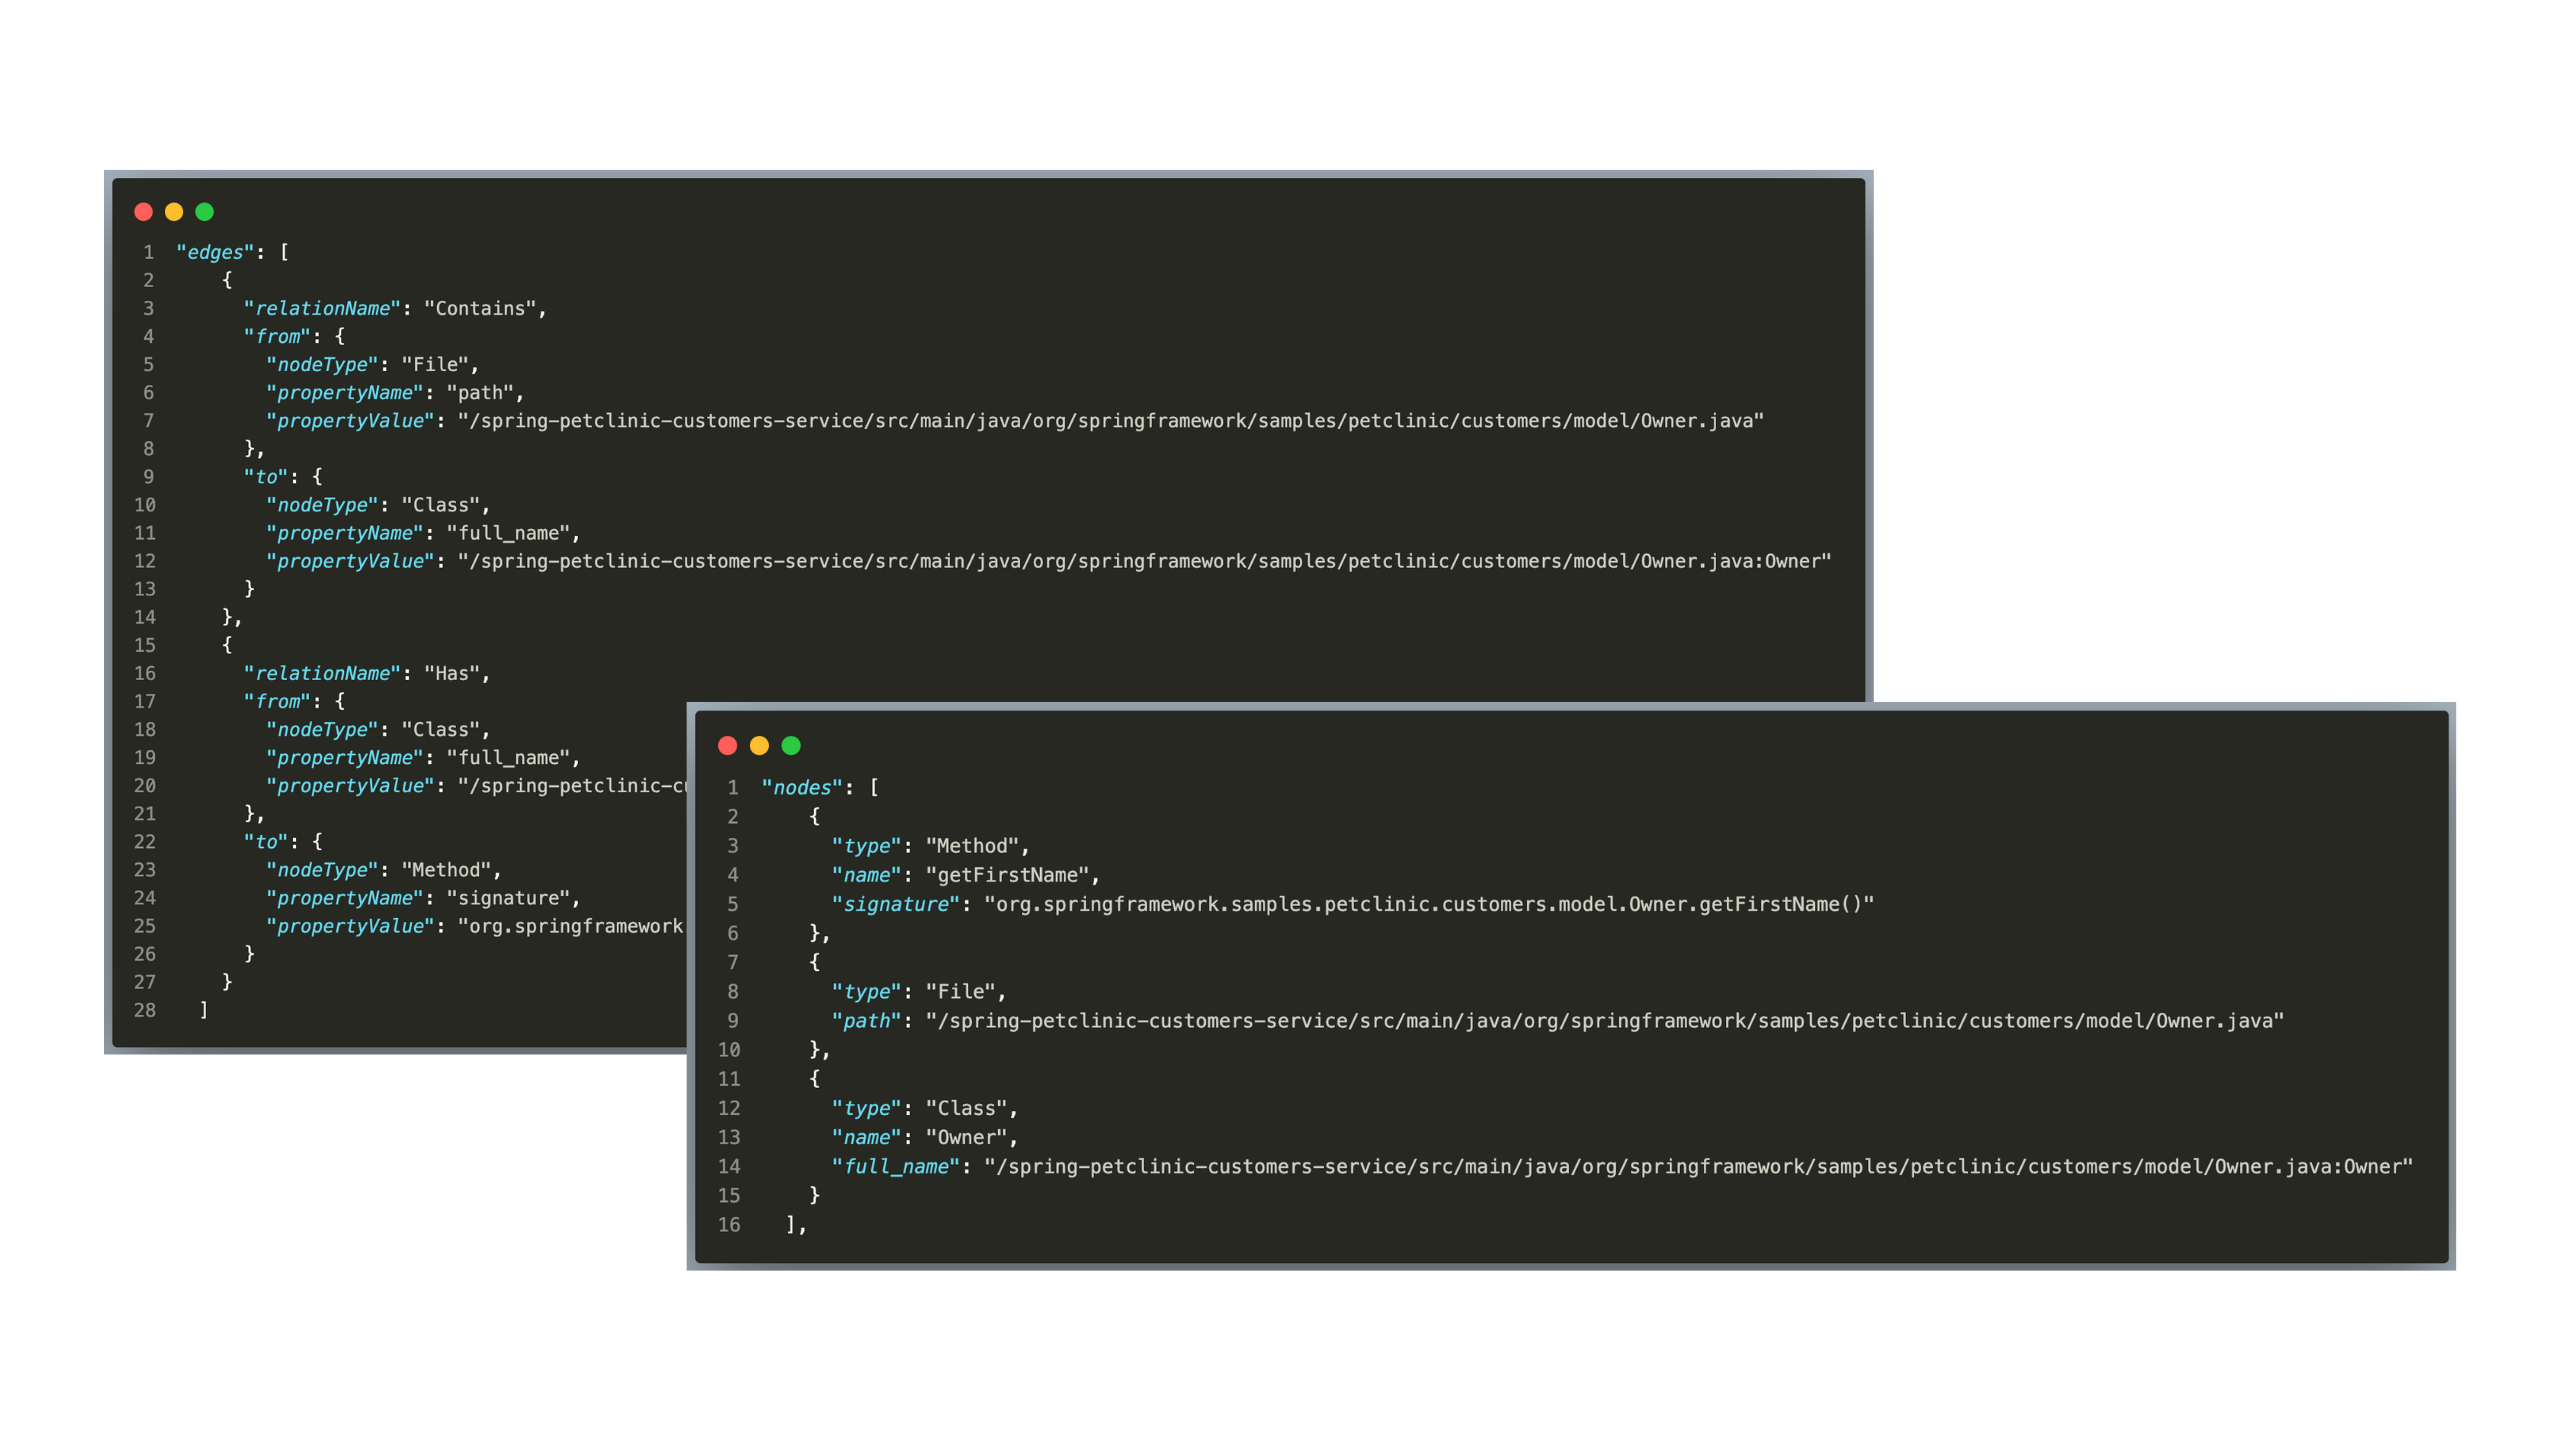
\includegraphics[width=1\textwidth]{figures/nodes_edges_example1.png}
    \caption{Example of Nodes and Edges array for author tracking JSON file}
    \label{fig:example_nodes_edges_author_tracking}
\end{figure}

\subsection{Implementation of probes related to microservices REST API endpoints}

In Section~\ref{ch3-sec:technical_validation_strategy}, we discussed a strategy to extract REST API endpoints from Java Spring Framework source code. The approach involves searching for relevant annotations and decorators in the source code and using them to identify endpoints. We apply this logic to extract the required information.  

In the implemented Python script, we first extract Java files from all services. Then, we use regular expressions to check if they contain annotations such as @RestController, @RequestMapping, @GetMapping, @PostMapping, and similar decorators. If a file includes these annotations, we extract the full route information and create class and endpoint nodes. This allows us to represent how a particular class maps to an endpoint through relational edges.

\begin{figure}[H]
    \centering
    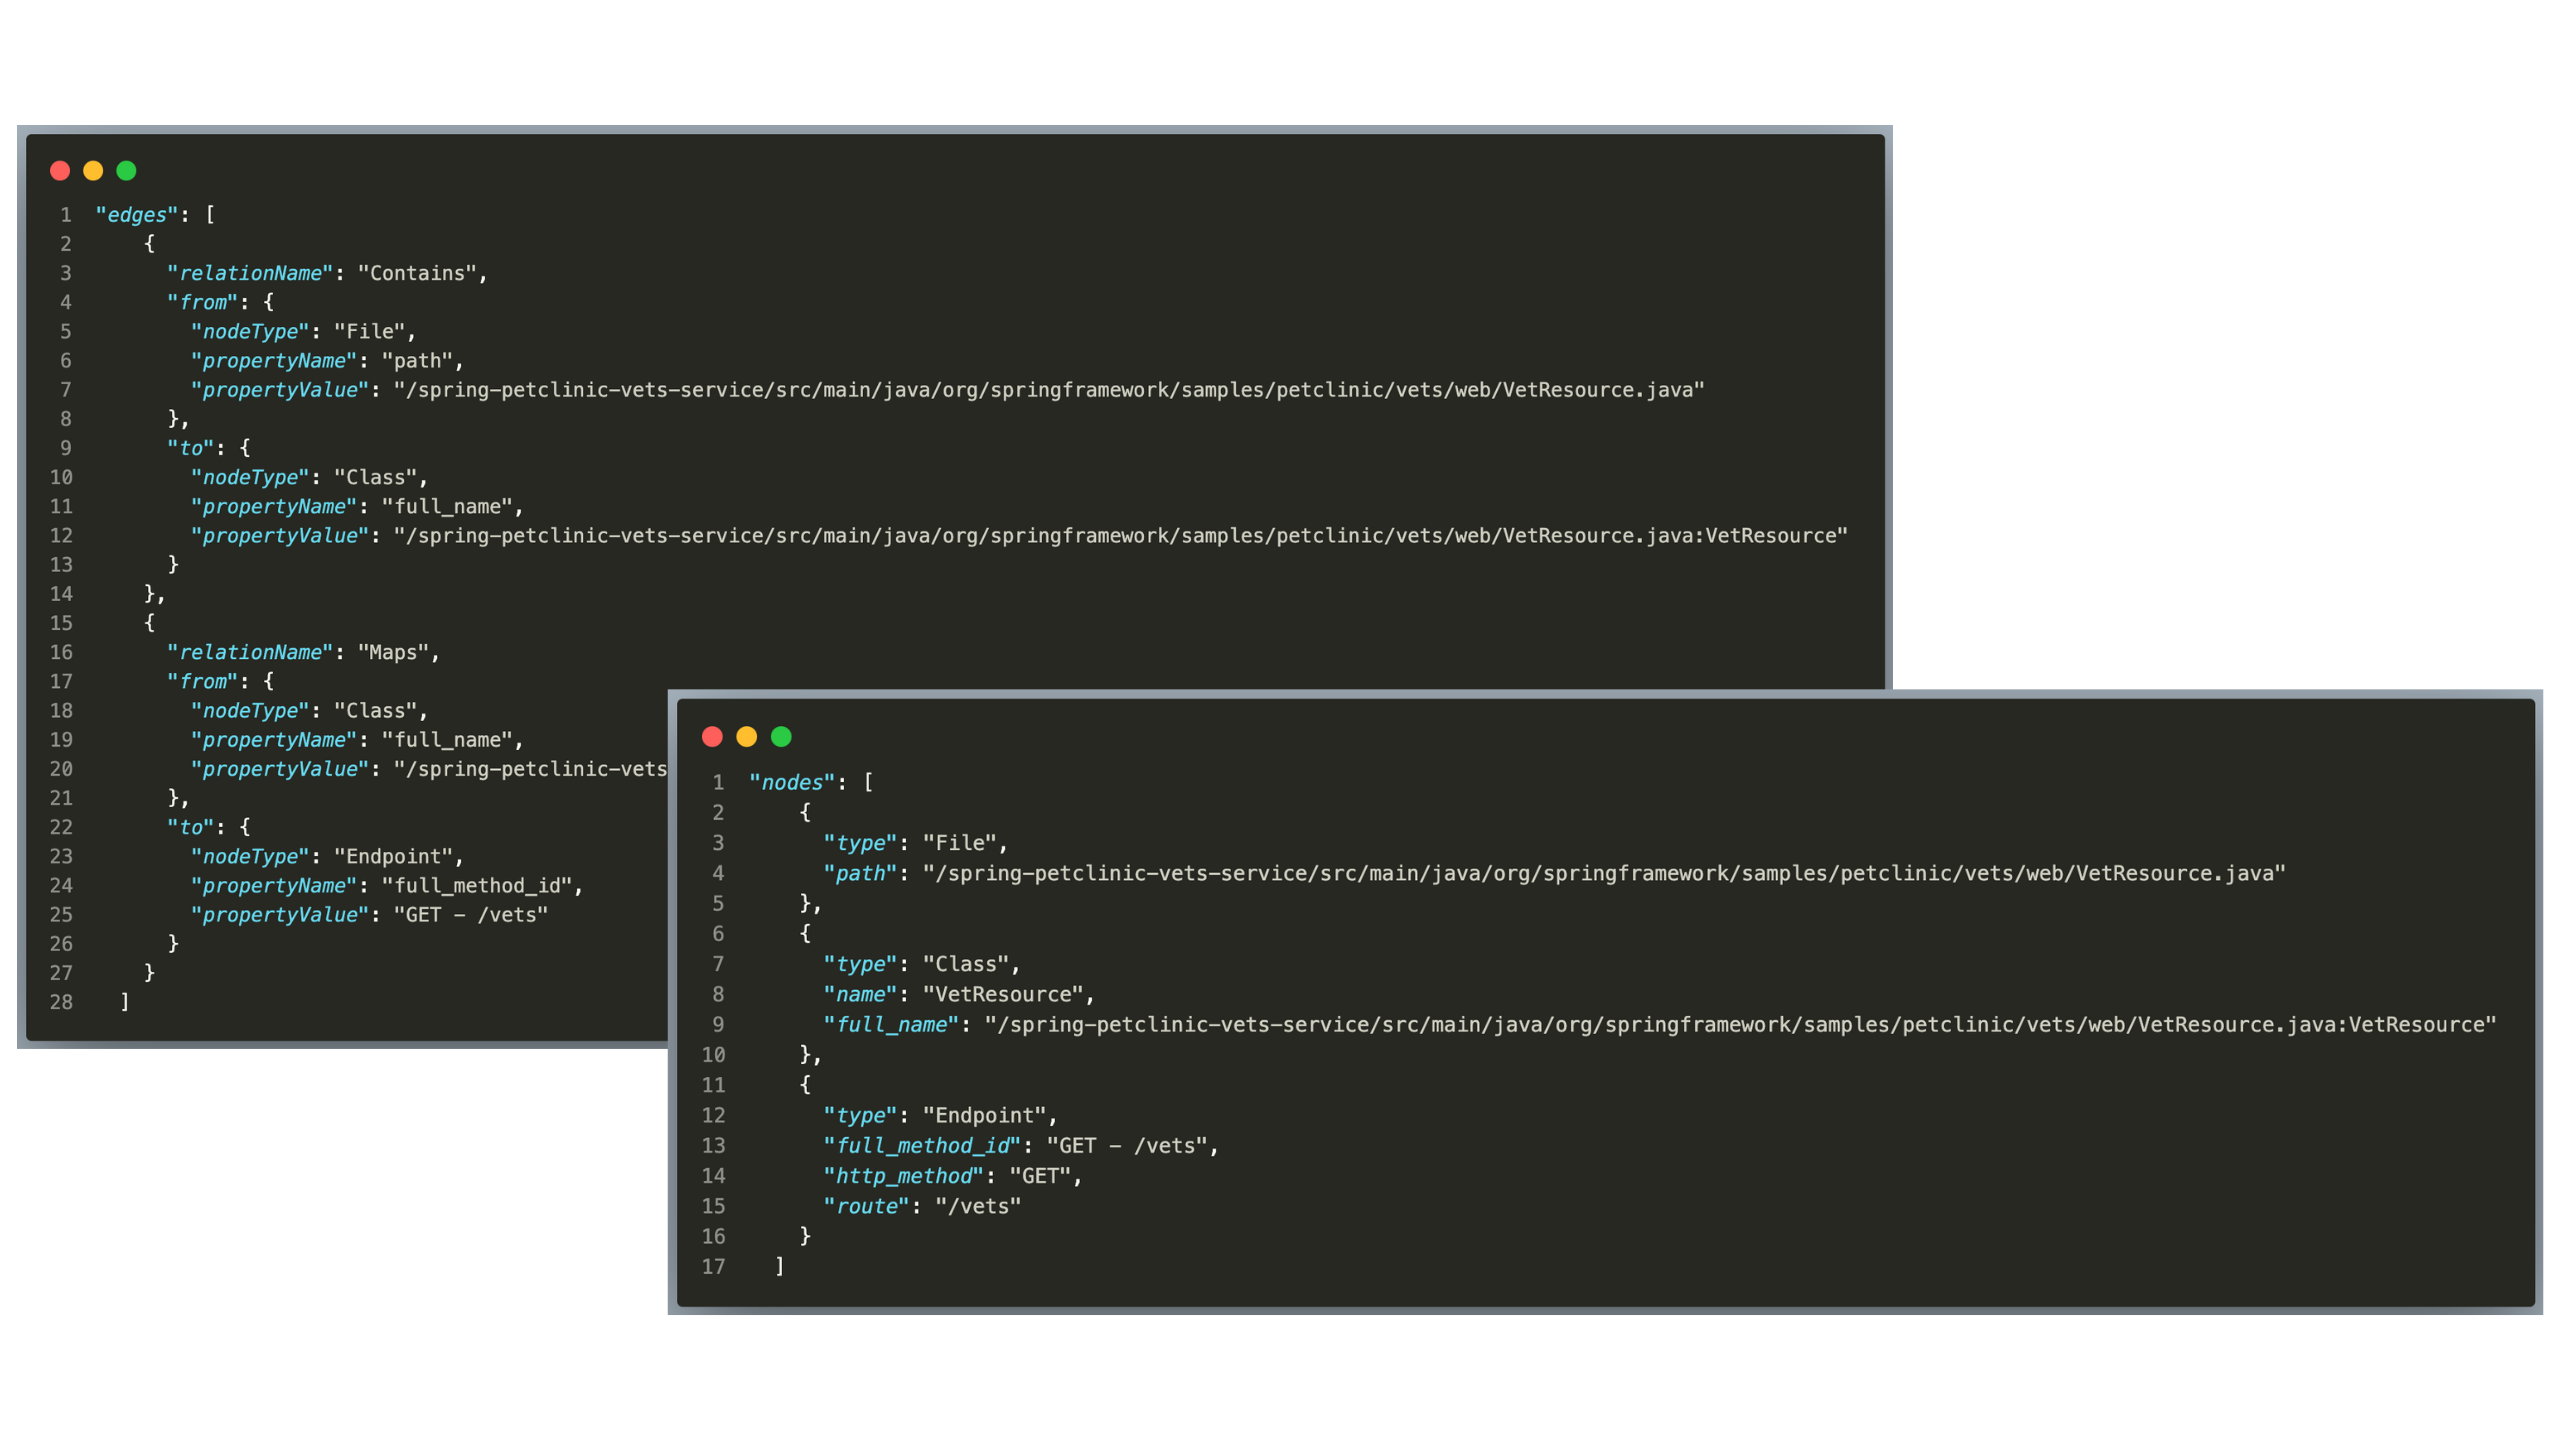
\includegraphics[width=1\textwidth]{figures/nodes_edges_example2.png}
    \caption{Example of Nodes and Edges array for REST API endpoints in services}
    \label{fig:example_nodes_edges_endpoints}
\end{figure}

\subsection{Implementation of probes related to java beans extraction}

Using a similar approach to extracting REST API endpoints, we can also extract Java beans from the source code. Java beans are created using specific annotations placed at the top of a class. These annotations indicate that the class is a Java bean, which will be managed by the Java Spring Framework.

In the Python script we have implemented, we search for @Component, @Service, @Repository, @Controller, and @Configuration annotations in the source code to identify beans.

Once the beans are found, we also extract their methods by searching for the @Bean annotation. In this script, we use javalang to parse methods when identifying bean methods, and Python regular expressions to find classes in the source code. After identifying the beans and their methods, we create their nodes using Python classes in our code. This allows us to establish relational edges between them.

\begin{figure}[H]
    \centering
    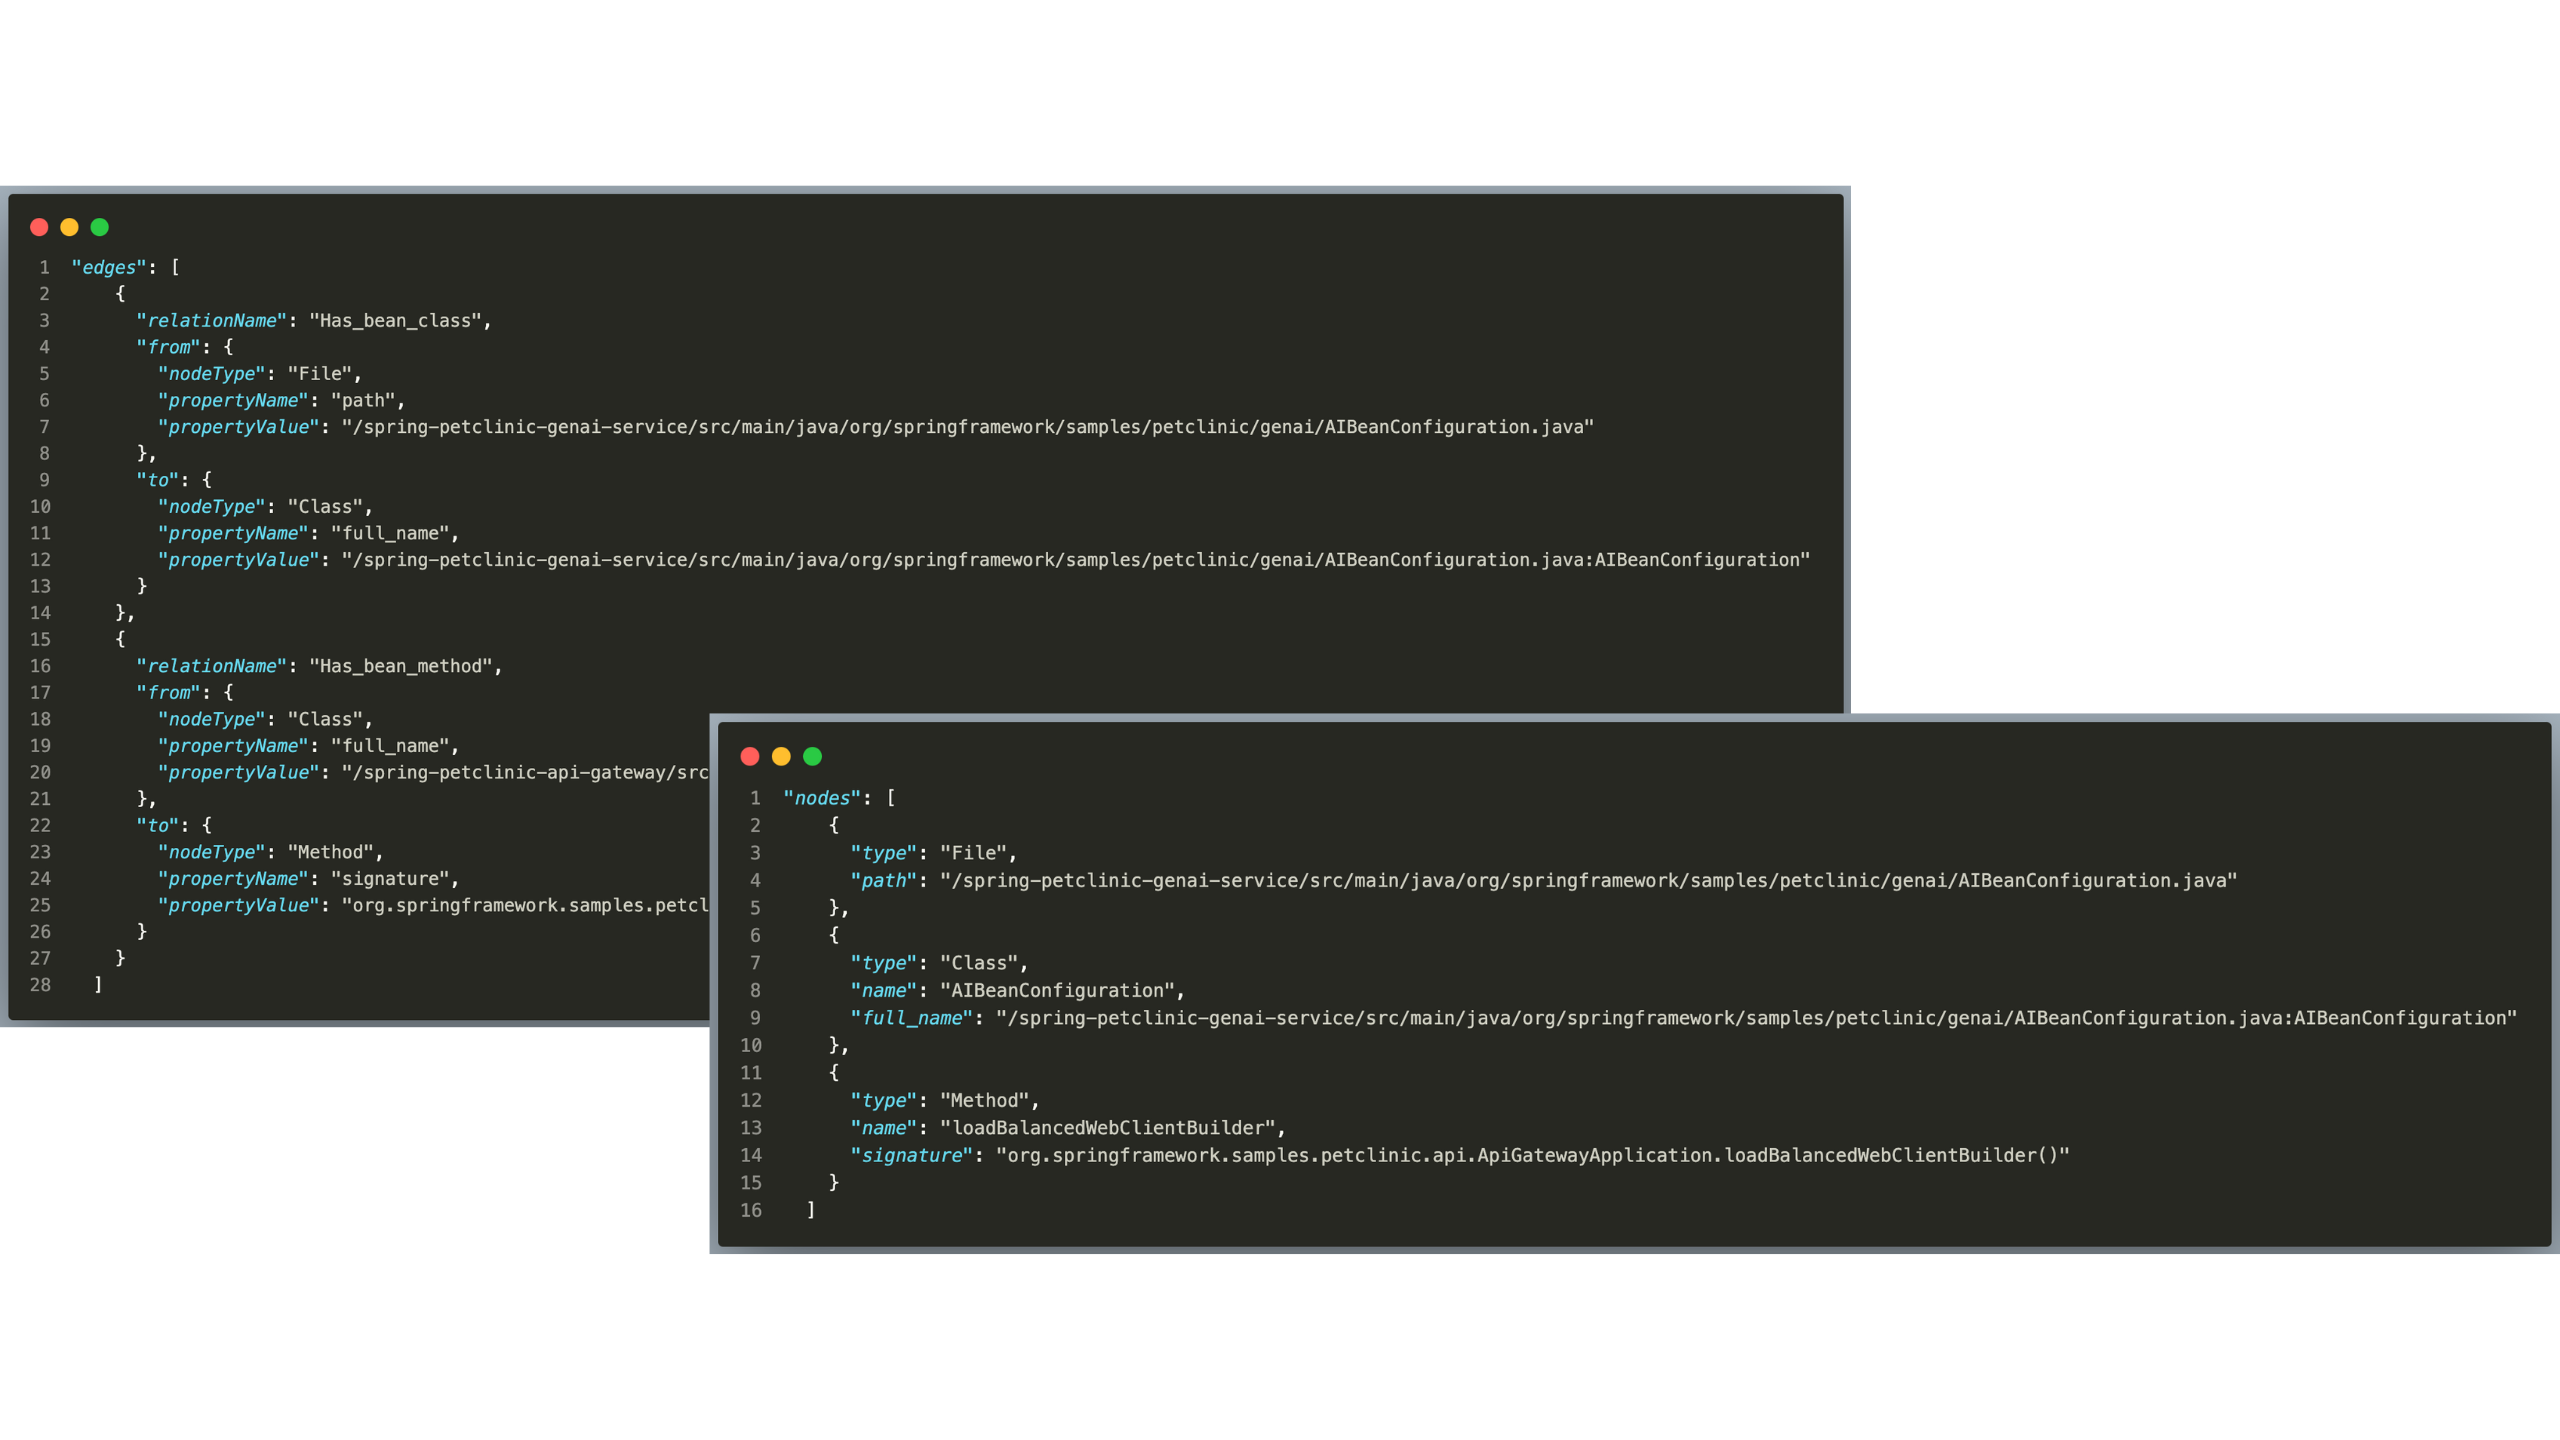
\includegraphics[width=1\textwidth]{figures/nodes_edges_example3.png}
    \caption{Example of Nodes and Edges array for Java beans JSON file}
    \label{fig:example_nodes_edges_java_beans}
\end{figure}

\subsection{Implementation of probes related to java dependencies extraction}

Java services have a Project Object Model (POM) file that contains information about the Maven project and how it is built. It is an XML file that includes a list of all project dependencies. We can use this file to extract dependencies and their versions.

In the Python script we have implemented, we use a lightweight Python XML parser~\citep{python-elementtree} for this purpose. We parse the XML file, extract the dependencies from each service, and create nodes and edges based on this information. When a dependency is found in the POM file, a node is created using the dependency class in our code. These nodes are then linked to each other using edges to represent relationships between dependencies.

\begin{figure}[H]
    \centering
    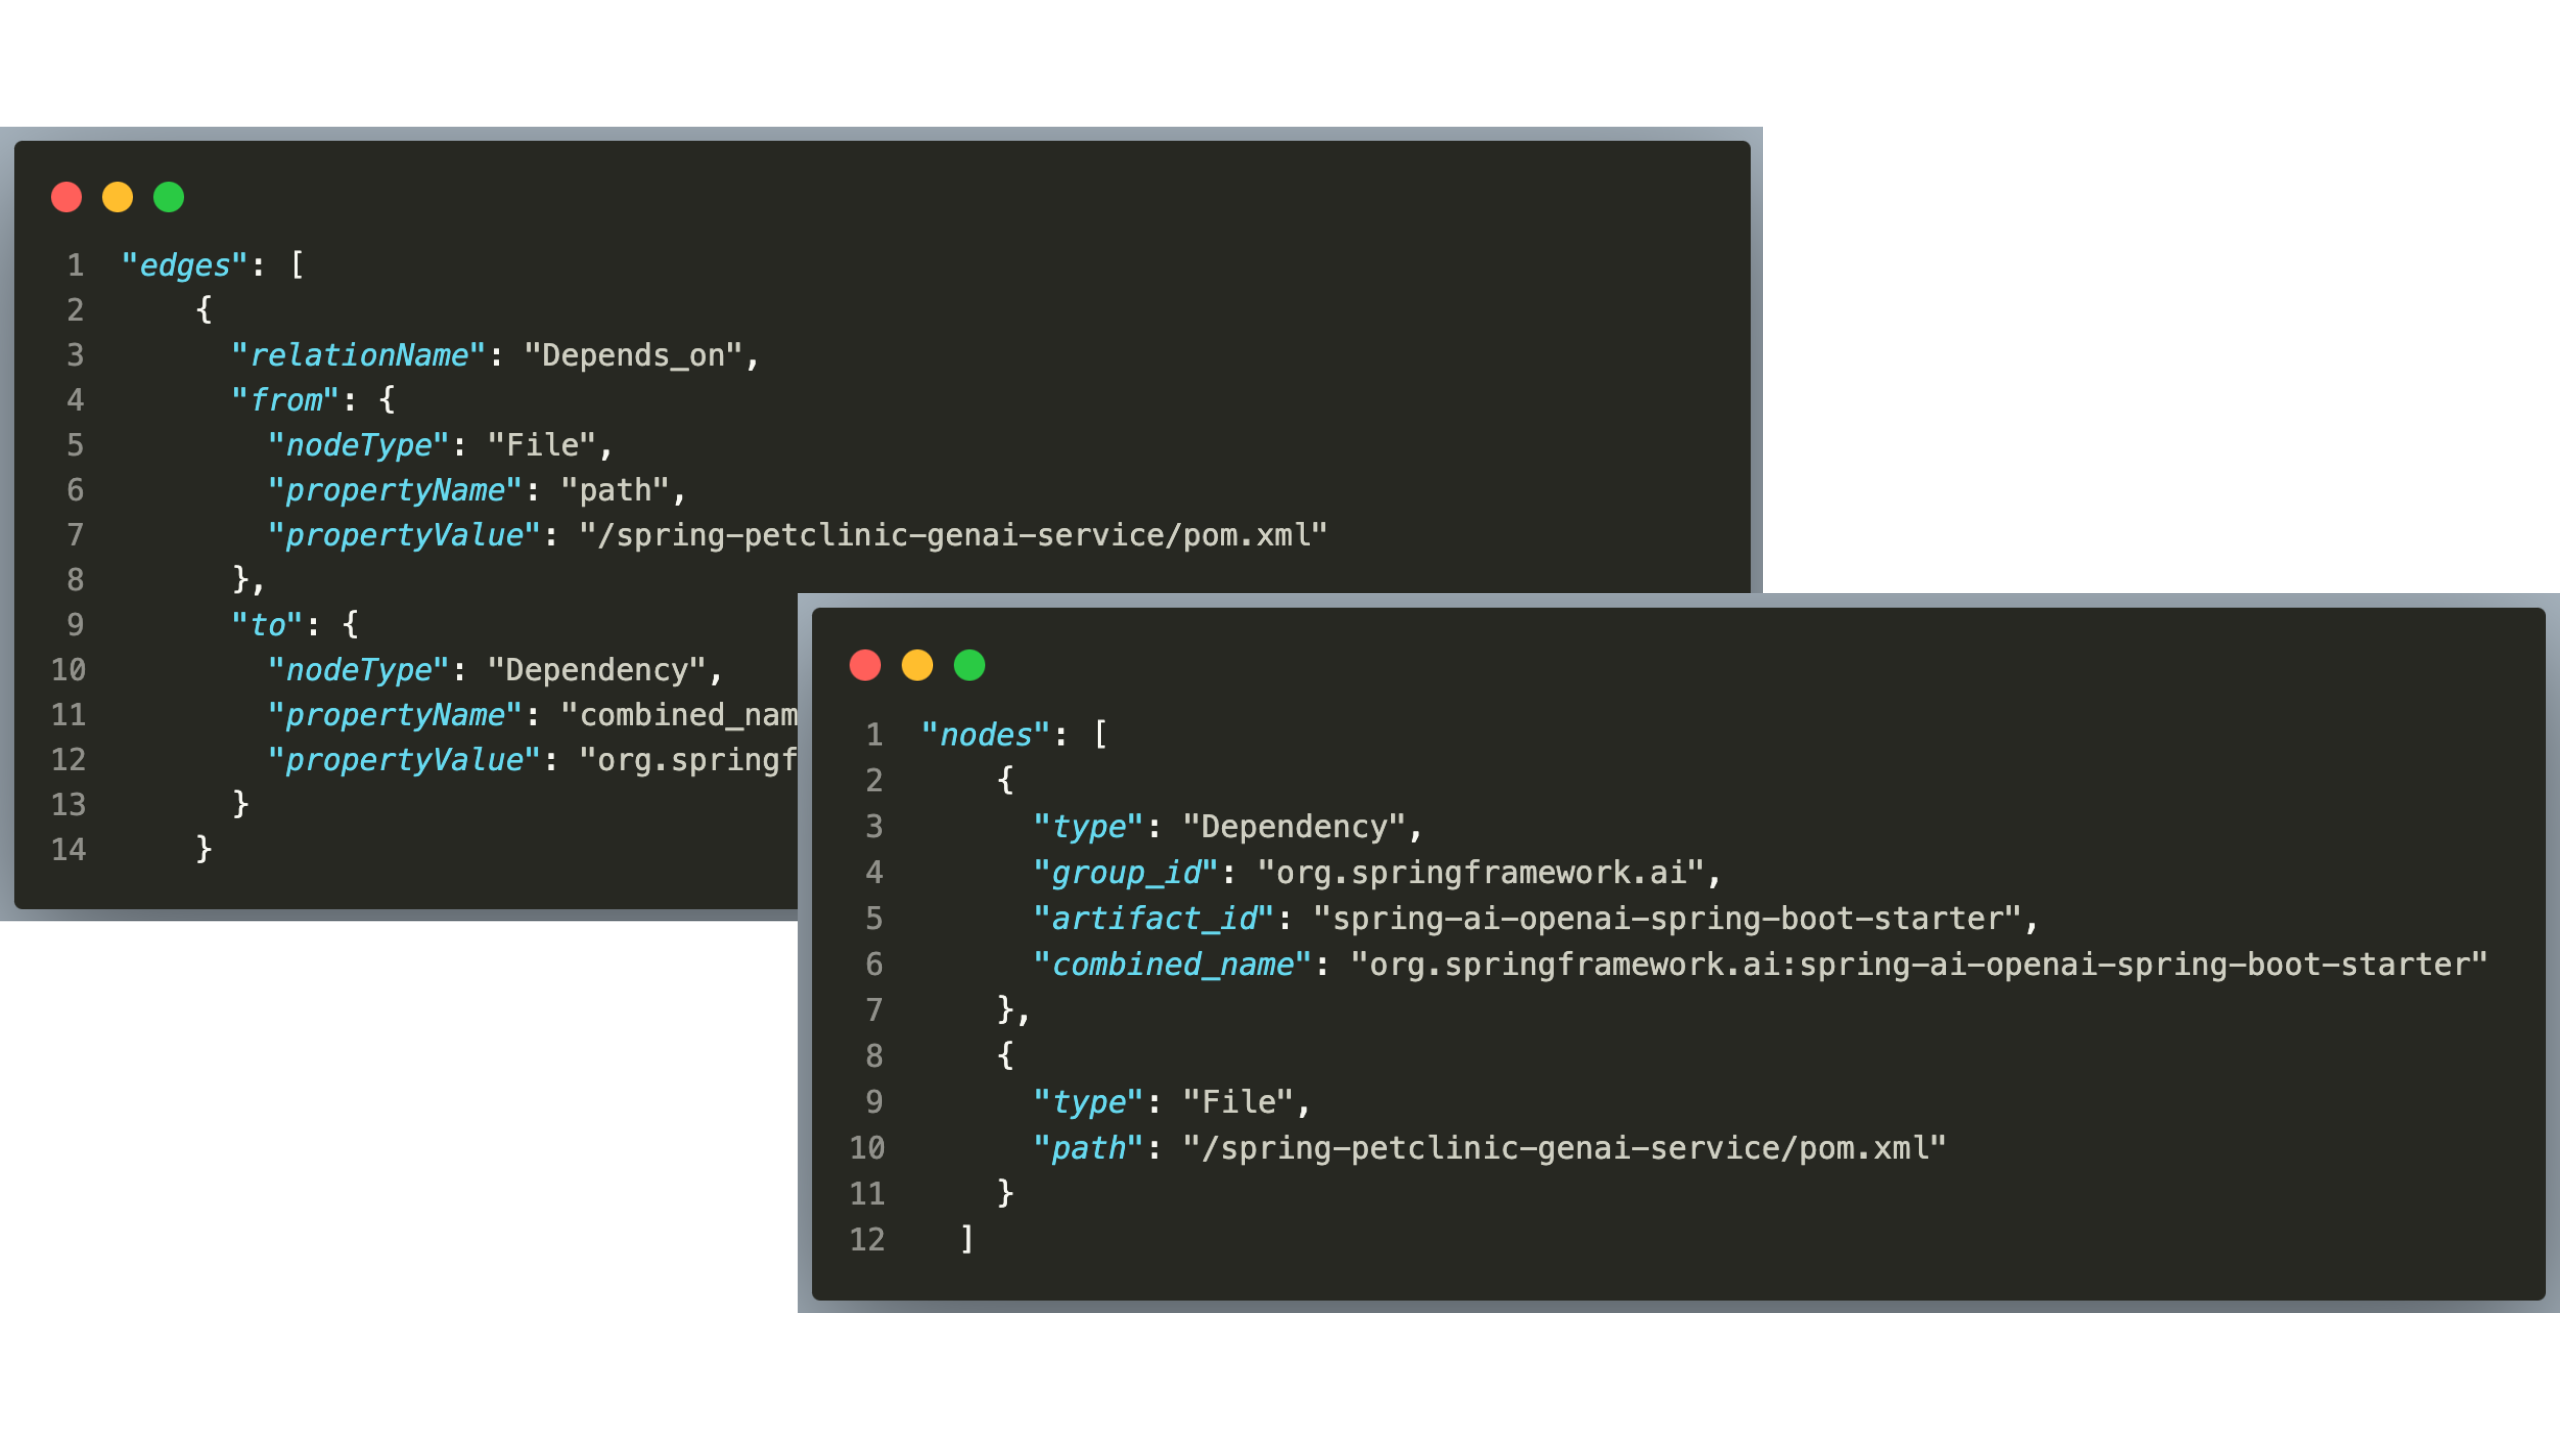
\includegraphics[width=1\textwidth]{figures/nodes_edges_example4.png}
    \caption{Example of Nodes and Edges array for Java dependencies JSON file}
    \label{fig:example_nodes_edges_java_dependencies}
\end{figure}

\subsection{Executor script and How it works}

We have a Python executor script that is responsible for running each probe script. To manage these probes, we use a file named ``probes\_list.py'', which contains a list of Python dictionaries. Each dictionary represents a probe and includes three key elements: runner\_command, probe\_file, and output\_file. The executor script iterates through this list, executing each probe and sending a POST request to the SST server to update it with the latest extracted data.  

One of the key advantages of this approach is that probes do not have to be written exclusively in Python. As long as a probe is placed in the `probes` folder and its corresponding runner command and probe file are specified in probes\_list.py, it can be executed in the same way as other probes. This flexibility allows for seamless integration of scripts written in different programming languages.  

The executor script ensures that the data sent to the SST server is always up to date, consistent, and valid. It takes the source directory of the target source code as a command-line argument, allowing users to specify the location of the project they want to analyze. Below is an example of how to run the script:

\begin{tcolorbox}[colback=gray!10, colframe=gray!20]
	python3 executor.py ---SOURCE\_DIR ``/Projects/spring-petclinic-microservices''
\end{tcolorbox}

This method ensures an efficient and automated way to extract and update data while maintaining consistency across different probes.